\chapter{Create an animation}
{ }\hfill\textbf{Level:} Medium\\ \\
This chapter presents two different themes with the goal of creating animation in \xlogo.
\section{Calculator's numbers}
\begin{center}
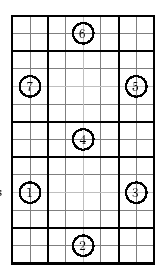
\includegraphics{pics/animation-chiffre.png}
\end{center}
\noindent This theme is based on the fact that every calculator's number could be drawn with the above schema:
\begin{itemize}
\item For example, to draw digit 4, we light rectangles 3,4,5,7.
\item To draw digit 8, we light rectangles 1,2,3,4,5,6,7.
\item To draw digit 3, we light rectangles 2,3,4,5,6.
\end{itemize}

\subsection{Filling a rectangular}
\begin{center}
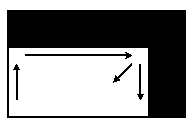
\includegraphics{pics/animation-rectangle.png}
\end{center}
\noindent If we want to draw a filled rectangle with dimensions 100 by 200, a first idea could be to draw a rectangle 100 by 200 then to draw a rectangle 99 by 199, then a rectangle 98 by 198 ... until the rectangle is fully filled.  \\
Let's begin by defining a rectangle with two variables corresponding to width and height
\begin{verbatim}
to rec :h :w
repeat 2[fd :h rt 90 fd :w rt 90]
end
\end{verbatim}
To fill our rectangle, we have to run:\\
\texttt{rec 100 200 rec 99 199 rec 98 198  ..... rec 1 101}\\ \\
Let's define a procedure for this filled rectangle.
\begin{verbatim}
to rectangular :h :w
rec :h :w
rectangular :h-1 :w-1
end
\end{verbatim}
We test \texttt{rectangular 100 200} and we can see there is a problem: The procedure doesn't stop when the rectangle has been filled, it continues infinitely! We must add a breakout test that will detect if width or height is equal to 0. When this condition is realized, we'll ask the program to stop with the primitive \texttt{stop}.
\begin{verbatim}
to rectangular :h :w
if or :h=0 :w=0 [stop]
rec :h :w
rectangular :h-1 :w-1
end
\end{verbatim}
Note: Instead of using the primitive \texttt{or}, it's possible to use the symbol |, the line becomes:
 \begin{center}
\texttt{if :h=0 | :w=0 [stop]}
\end{center}
\subsection{The program}
\noindent We must reuse the precedent filled rectangle:
\begin{verbatim}
to rectangular :h :w
if or :h=0 :w=0 [stop]
rec :h :w
rectangular :h-1 :w-1
end
\end{verbatim}
We suppose that the turtle starts from the bottom left corner. We're going to define a procedure called \texttt{number} depending on 7 arguments \texttt{:a}, \texttt{:b}, \texttt{:c}, \texttt{:d}, \texttt{:e}, \texttt{:f}, \texttt{:g}. When \texttt{:a} is equal to 1, we draw the rectangle 1. If \texttt{:a} is equal to 0, we don't draw this rectangle. Here is the main idea.\\ \\
\textbf{The code}:
\begin{verbatim}
to number :a :b :c :d :e :f :g
# we draw the rectangular 1
if :a=1 [rectangular 160 40]
# we draw the rectangular 2
if :b=1 [rectangular 40 160]
penup right 90 forward 120 left 90 pendown
# we draw the rectangular 3
if :c=1 [rectangular 160 40]
penup forward 120 pendown
# we draw the rectangular 5
if :e=1 [rectangular 160 40]
# we draw the rectangular 4
left 90 penup back 40 pendown
if :d=1 [rectangular 160 40]
# we draw the rectangular 6
right 90 penup forward 120 left 90 pendown
if :f=1 [rectangular 160 40]
# we draw the rectangular 7
penup forward 120 left 90 back 40 pendown 
if :g=1 [rectangular 160 40]
end

\end{verbatim}
\subsection{Creating an animation}
\noindent In this part, we'll define a countdown from 9 to 0.
\begin{verbatim}
to countd
clearscreen hideturtle number 0 1 1 1 1 1 1 wait 60
clearscreen hideturtle number 1 1 1 1 1 1 1 wait 60
clearscreen hideturtle number 0 0 1 0 1 1 0 wait 60
clearscreen hideturtle number 1 1 1 1 0 1 1 wait 60
clearscreen hideturtle number 0 1 1 1 0 1 1 wait 60
clearscreen hideturtle number 0 0 1 1 1 0 1 wait 60
clearscreen hideturtle number 0 1 1 1 1 1 0 wait 60
clearscreen hideturtle number 1 1 0 1 1 1 0 wait 60
clearscreen hideturtle number 0 0 1 0 1 0 0 wait 60
clearscreen hideturtle number 1 1 1 0 1 1 1 wait 60
end
\end{verbatim}
Little problem: There is a flickering effect during each number drawing. To make the animation fluid, we're going to use the three primitives \texttt{animation}, \texttt{stopanimation} and \texttt{repaint}.\\
\begin{itemize}
\item \texttt{animation} enables the mode ``animation''. The turtle stops drawing on the screen but remembers all changes in cache. To display the image, it's necessary to use the primtive \texttt{repaint}.
\item  \texttt{stopanimation} returns to the classic drawing mode.
\end{itemize}
Here is the new code for this procedure:
\begin{verbatim}
to countd
# Enables animation mode
animation
clearscreen hideturtle number 0 1 1 1 1 1 1 repaint wait 60
clearscreen hideturtle number 1 1 1 1 1 1 1 repaint wait 60
clearscreen hideturtle number 0 0 1 0 1 1 0 repaint wait 60
clearscreen hideturtle number 1 1 1 1 0 1 1 repaint wait 60
clearscreen hideturtle number 0 1 1 1 0 1 1 repaint wait 60
clearscreen hideturtle number 0 0 1 1 1 0 1 repaint wait 60
clearscreen hideturtle number 0 1 1 1 1 1 0 repaint wait 60
clearscreen hideturtle number 1 1 0 1 1 1 0 repaint wait 60
clearscreen hideturtle number 0 0 1 0 1 0 0 repaint wait 60
clearscreen hideturtle number 1 1 1 0 1 1 1 repaint wait 60
# back to classic mode
stopanimation
end
\end{verbatim}
\section{Second animation: The growing man}
\begin{center}
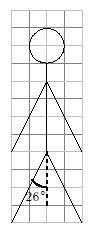
\includegraphics{pics/animation-bonhomme.png}
\end{center}
First, we'll define a procedure \texttt{man} that draws the above schema. We use a variable to reproduce it at different scales 
\begin{verbatim}
to man :c
left 154 forward 44*:c back 44*:c 
left 52 forward 44*:c back 44*:c 
left 154 forward 40*:c
left 154 forward 44*:c back :c*44 
left 52 forward 44*:c back :c*44 
left 154 forward 10*:c
left 90 repeat 180[forward :c/2 right 2] right 90
end
\end{verbatim}
Now, we'll create an animation that will make the man grow. To realize this, we'll draw \texttt{man 0.1}, then \texttt{man 0.2} \texttt{man 0.3} ... until \texttt{man 5}. Between each man, we'll erase the screen. We obtain two different procedures:
\begin{verbatim}
to man :c
left 154 forward 44*:c back 44*:c 
left 52 forward 44*:c back 44*:c 
left 154 forward 40*:c
left 154 forward 44*:c back :c*44 
left 52 forward 44*:c back :c*44 
left 154 forward 10*:c
left 90 repeat 180[forward :c/2 right 2] right 90
if :c=5[stop]
cs ht man :c+0.1
end

to go
cs ht
man 0
end
\end{verbatim}
Finally to make the animation fluid, we'll use animation mode and the primitive \texttt{repaint}.
\begin{verbatim}
to man :c
left 154 forward 44*:c back 44*:c 
left 52 forward 44*:c back 44*:c 
left 154 forward 40*:c
left 154 forward 44*:c back :c*44 
left 52 forward 44*:c back :c*44 
left 154 forward 10*:c
left 90 repeat 180[forward :c/2 right 2] right 90
repaint
if :c=5[stop]
cs ht man :c+0.1
end

to go
cs ht animation
man 0
stopanimation
end
\end{verbatim}
\textbf{Note: } Here, the procedure \texttt{man} is recursive. In aother way, we could use the primitive \texttt{for} to make the variable \texttt{:c} from 0.1 to 5. Here is the program:
\begin{verbatim}
to man :c
cs left 154 forward 44*:c back 44*:c 
left 52 forward 44*:c back 44*:c 
left 154 forward 40*:c
left 154 forward 44*:c back :c*44 
left 52 forward 44*:c back :c*44 
left 154 forward 10*:c
left 90 repeat 180[forward :c/2 right 2] right 90
repaint
end

to go
ht animation
for [c 0 5 0.1][man :c]
stopanimation
end
\end{verbatim}